\section{Architektura LOD}
\label{sec-LODarchitecture}
Realizace systému vykreslování a řízení úrovní jednotlivých stromů reflektuje možnosti současných grafických karet. Jelikož je objem dat zpracovávaný v každém snímku relativně velký a současně se z velké části nemění, lze tyto neměnná data přesunout do paměti GPU a tím i zefektivnit jejich zpracování. Ušetří se tím zbytečné přenosy po sběrnici mezi hlavní pamětí a pamětí grafické karty. Tento přístup je v dnešní době standardem a OpenGL ho samozřejmě podporuje ve formě tzv. \emph{Vertex Buffer Objects} (VBO), což je struktura obsahující data příslušná vrcholům jako jejich atributy (např.: pozice, normála, barva, atd.). 

\begin{figure}[!hbt]
\begin{center}
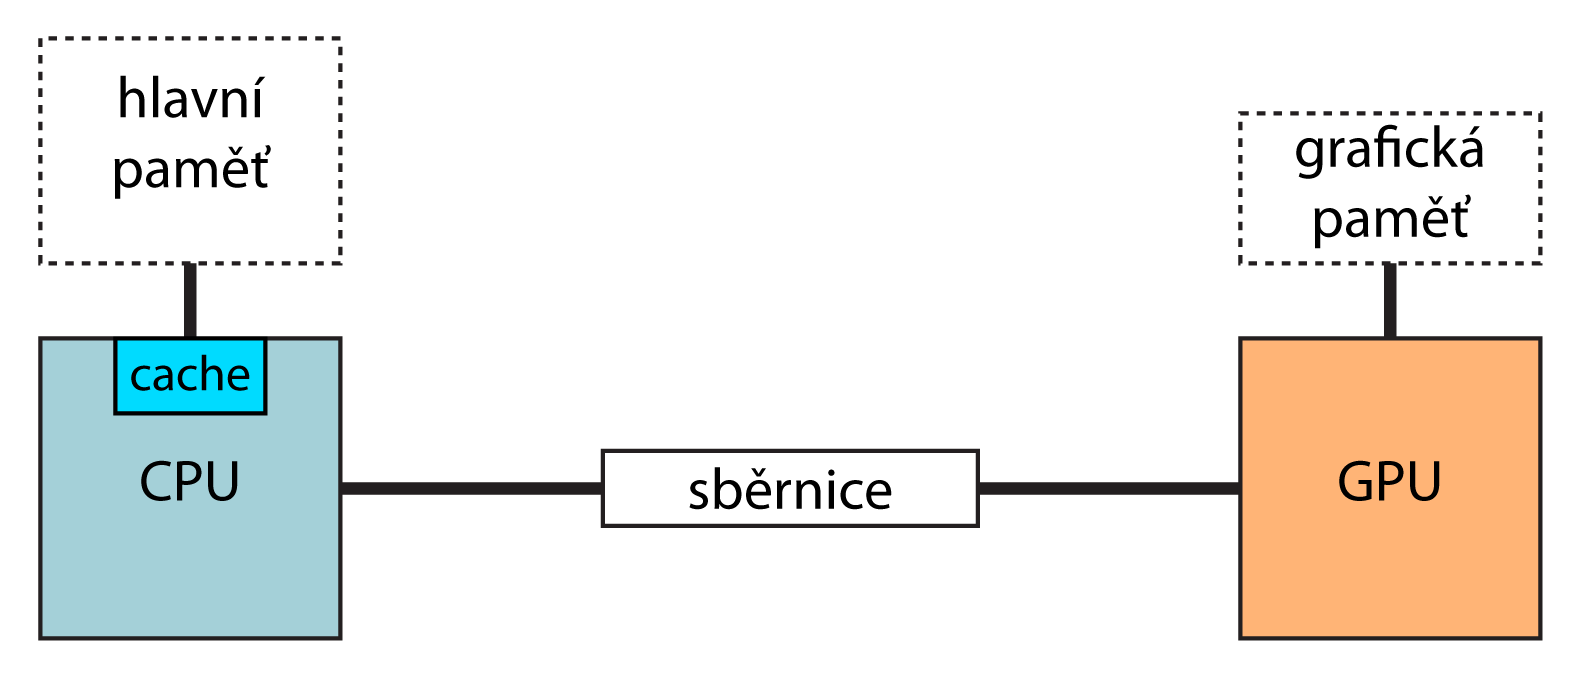
\includegraphics[width=0.75\textwidth]{./figures/CPUaGPU.png}
\end{center}
\caption[Různé druhy pamětí]%
{Různé druhy pamětí: hlavní paměť při CPU a grafická paměť na GPU. Přenos dat po sběrnici může mít negativní vliv na výkon.
\label{fig:CPUaGPU}
}
\end{figure}

Tato data mohou být umístěna jak v hlavní paměti, tak i v paměti GPU. Požadavek na umístění těchto dat lze vyjádřit při jejich zápisu do VBO příkazem 
\begin{verbatim}glBufferData(..., const GLvoid *  data, GLenum  usage)\end{verbatim}
Parametr \lineCode{usage} definuje povahu dat. Např. hodnota \lineCode{GL\_STATIC\_DRAW} informuje OpenGL o tom, že data se nebudou měnit a je tedy vhodné přesunout je do paměti GPU . Podle konkrétní implementace OpenGL a možností grafického hardware je tedy tedy tento přesun proveden, či je umístění dat jinak optimalizováno. Naproti tomu hodnota \lineCode{GL\_STREAM\_DRAW} naznačuje, že data budou v každém snímku změněna a přenos mezi CPU a GPU nelze ušetřit. Proto budou v takovém případě data raději v hlavní paměti.

Kromě VBO existuje ještě obdobný konstrukt pro uložení indexů indexované geometrie - tzv. \emph{Element Buffer Objects} (EBO). Indexovaná geometrie je výhodná zejména v případě, že se atributy vrcholů nemění a vrcholy jsou použity v rámci tvorby geometrie vícekrát (např. vrchol je společný pro mnoho trojúhelníků)

Protože se předpokládá zobrazení více instancí téhož stromu, jeví se jako přirozené využít techniky \emph{instancování na GPU}, která vytváří jednotlivé instance dynamicky až v rámci hardwaru. Tato technika se vyplácí zejména pro zpracování a zobrazování většího počtu instancí. Jeví se tedy jako vhodné, využít ji pro zobrazování zejména instancí s nižším LOD (LOD1 a LOD2), kterých je typicky řádově více než instancí nejvyššího detailu. Myšlenka instancování na GPU je prostá. Pokud se instance vzájemně liší pouze několika globálními parametry (pozice a orientace ve scéně, příp. další atributy) není třeba každou instanci vykreslovat zvláštním příkazem. Místo toho je typicky využit příkaz:
\begin{verbatim}glDrawElementsInstanced(..., GLsizei pocetInstanci)\end{verbatim}
Ten vykreslí zadaný počet instancí připojené indexované geometrie. Jelikož je však třeba jednotlivé instance správně umístit do scény a přiřadit jim i další specifické parametry, je třeba předat konkrétní instanci příslušná data. K tomu účelu se využívá princip tzv. \emph{instančních atributů}. Narozdíl od běžných atributů, které přísluší jednotlivým vrcholům (typicky normála, tangenta, texturovací souřadnice apod.), instanční atributy jsou stejné pro všechny vrcholy dané instance, ale liší se mezi instancemi. Toto chování lze zajistit příkazem:
\begin{verbatim}glVertexAttribDivisor(GLuint attribDesc, GLuint divisor)\end{verbatim}
Parametr \lineCode{divisor} určuje, pro kolik instancí bude atribut popsaný \lineCode{attribDesc} stejný. Hodnota $0$ vrací chování zpět na standardní - tedy atributy se různí pro jednotlivé vrcholy.
Instanční atributy je dobré uložit taktéž do VBO. Jelikož implicitně se všechny instance vykreslí díky použití stejných dat na stejnou pozici ve scéně, je nutné ve vertex shaderu transformovat všechny vrcholy dané instance příslušným způsobem. Z toho důvodu se jako jeden z instančních atributů předává i instanční transformační matice. Pořadí, v jakém jsou předány instanční atributy, určuje i pořadí vykreslování jednotlivých instancí.

Pro realizaci aplikace pracující s LOD jsou výše zmíněné možnosti zásadní. Jelikož je nutné v každém snímku určit pro každou instanci v jakém LOD se bude vykreslovat a to závisí v tomto případě na vzdálenosti od pozorovatele, jsou instance zpracovávány postupně a jsou přiřazeny do jedné ze zobrazovacích front (viz obr. \ref{fig:InstanceQueues}). 
\begin{figure}[!hbt]
\begin{center}
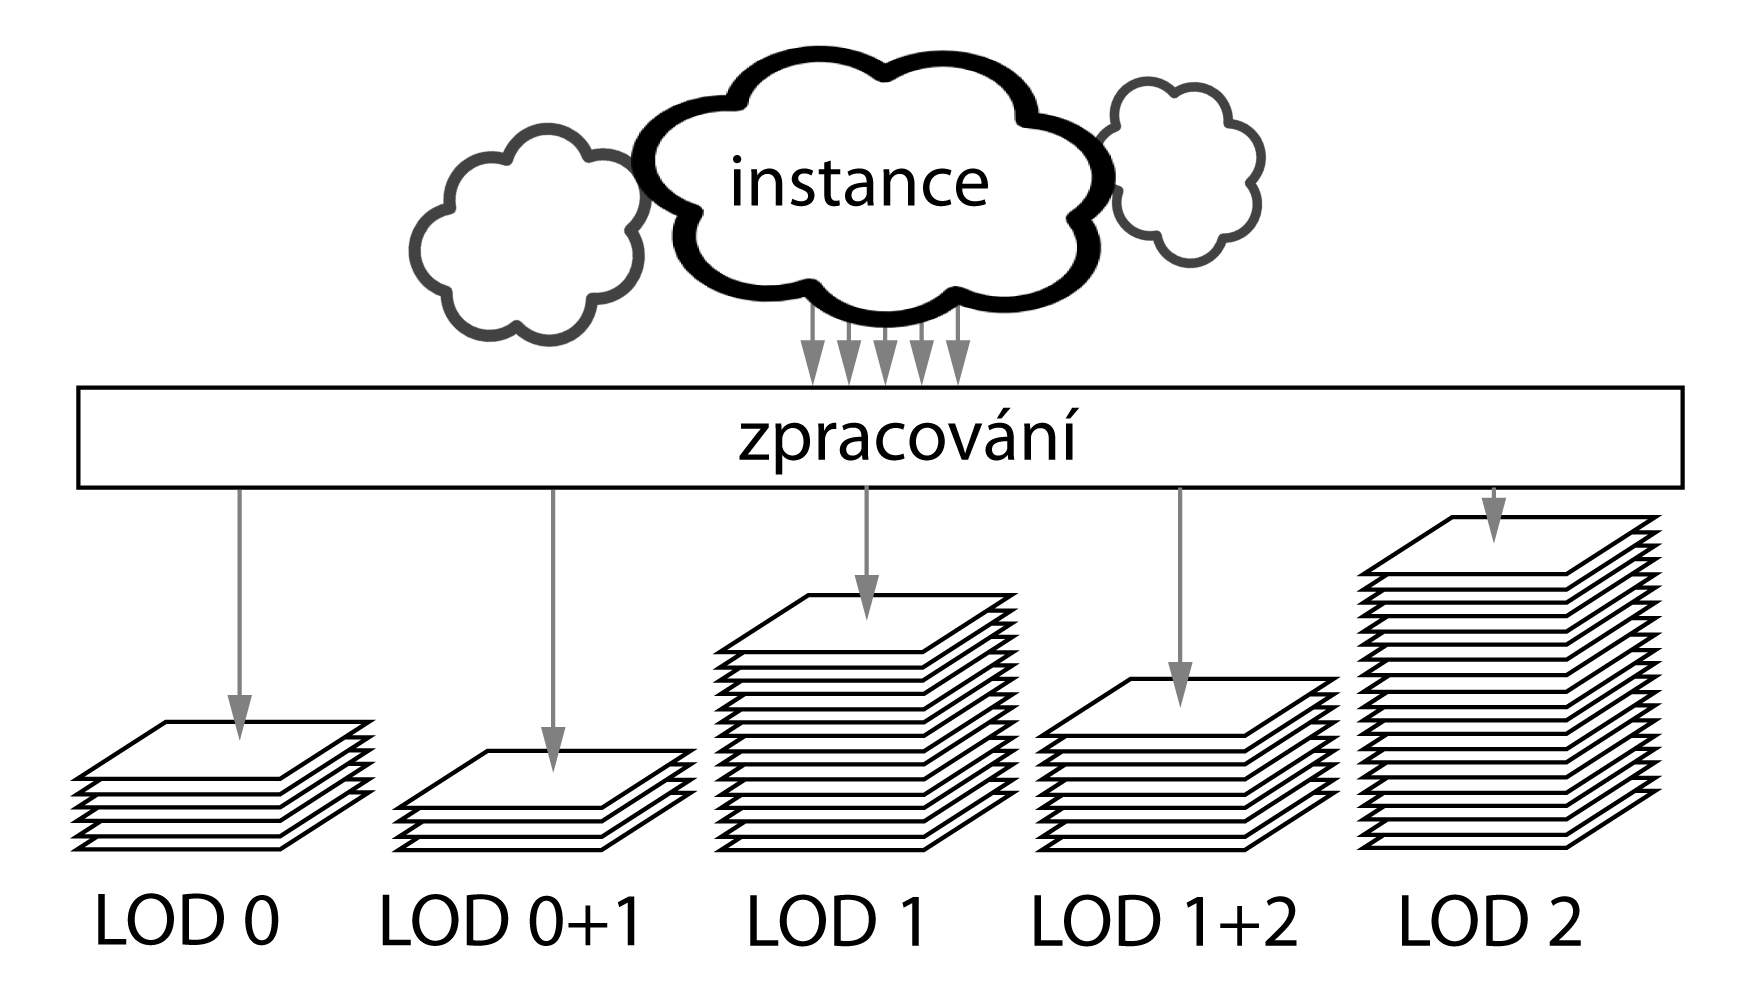
\includegraphics[width=0.5\textwidth]{./figures/renderQueuesA.png}
\end{center}
\caption[Fronty instancí]%
{Fronty instancí. LOD0 jsou instance v nejvyšším stupni detailu. Fronta LOD0+1 představuje instance v přechodu mezi úrovněmi LOD0 a LOD1. Obdobně i pro LOD2.
\label{fig:InstanceQueues}
}
\end{figure}
Některé instance pak lze vyřadit ze zobrazovacího procesu třeba proto, že neleží v prostoru aktuálního pohledu\footnote{stromy v těsném okolí pozorovatele ale mohou vrhat stín, a proto jsou zachovány} (např. leží za pozorovatelem). 

Instancím, které jsou pro daný pohled právě v přechodu mezi různými stupni LOD, je v rámci zpracování určena fáze přechodu a podle \cite{GIEGL-2007-UNP} jsou zobrazeny. V pseudokódu lze tento proces popsat následujícím způsobem:
\begin{verbatimtab}[4]
function makeTransition(float phase, Tree instance){
	float alpha1;
	float alpha2;
	if (phase<0.5){
		alpha1 = 1;	
		alpha2 = 2*phase;
		disableDepthBufferWrite();
			instance.drawLOD_B(instance, alpha2);
		enableDepthBufferWrite();
		instance.drawLOD_A(instance, alpha1);					
	} else {			
		alpha1 = 2*(1-phase);
		alpha2 = 1;	
		instance.drawLOD_B(instance, alpha2);	
		disableDepthBufferWrite();
			instance.drawLOD_A(instance, alpha1);
		enableDepthBufferWrite();	
	} 
}
\end{verbatimtab}

Kvůli průhlednosti, která hraje důležitou roli u nižších úrovní detailu, a která není implicitně řešena v rámci OpenGL, je nutné provádět vykreslování v pořadí od vzdálených instancí k bližším. Z toho důvodu je třeba provádět v rámci zpracování rychlé řazení instancí před vykreslením každého snímku \footnote{předpokládáme-li změnu pozice a pohledu pozorovatele}. Důležitý je fakt, že mezi následujícími snímky je zachována určitá koherence. Instance, které jsou v seřazeném pořadí v jednom snímku blízko sebe, budou nejspíš kdesi blízko sebe i ve snímku následujícím. S výhodou tedy lze použít částečného řazení s nižší (lineární) časovou složitostí. V tomto případě je využito jednoho průchodu algoritmu známého jako \emph{bubble-sort} (dále jen \emph{lazy-sort} neboli \emph{líné řazení}). Toto řazení funguje na úrovni jednotlivých instancí a poskytuje uspokojivé výsledky. 
Fronty instancí LOD1 a LOD2 jsou následně vykreslovány pomocí instančního zobrazování. Ostatní fronty, u kterých se předpokládá, že neobsahují tolik položek, jsou vykreslovány po jednotlivých instancích.
